\documentclass[12 pt]{article}
\usepackage[utf8]{inputenc}
\usepackage{matlab-prettifier}
\usepackage[portuguese]{babel}
\usepackage{indentfirst}
\usepackage{graphicx}
\usepackage{float}
\usepackage{subcaption}
\usepackage[font=small,labelfont=bf]{caption}
\definecolor{mygreen}{RGB}{28,172,0} % color values Red, Green, Blue
\definecolor{myyellow}{rgb}{1.0, 1.0, 0.8}
\usepackage{mathtools}
\usepackage{multirow}
\usepackage{comment}
\usepackage{xcolor}
\usepackage{colortbl}
\usepackage[normalem]{ulem}               % to striketrhourhg text
\usepackage{amsmath}
\usepackage{amsfonts}
\newcommand\redout{\bgroup\markoverwith
{\textcolor{red}{\rule[0.5ex]{2pt}{0.8pt}}}\ULon}
\renewcommand{\lstlistingname}{Código}% Listing -> Algorithm
\renewcommand{\lstlistlistingname}{Lista de \lstlistingname s}% List of Listings -> List of Algorithms
\usepackage{enumitem}
\usepackage[top=3cm,left=2cm,bottom=2cm, right=2cm]{geometry}

% Configuração para destacar a sintaxe do Python
\lstset{ 
    language=Python,                     % A linguagem do código
    backgroundcolor=\color{myyellow}, % A cor do fundo 
    basicstyle=\ttfamily\footnotesize,   % O estilo do texto básico
    keywordstyle=\color{blue},           % Cor das palavras-chave
    stringstyle=\color{red},             % Cor das strings
    commentstyle=\color{mygreen},          % Cor dos comentários
    numbers=left,                        % Números das linhas à esquerda
    numberstyle=\tiny\color{gray},       % Estilo dos números das linhas
    stepnumber=1,                        % Número de linhas entre os números das linhas
    frame=single,                        % Moldura ao redor do código
    breaklines=true,                     % Quebra automática das linhas longas
    captionpos=t,                        % Posição da legenda
    showstringspaces=false               % Não mostra espaços em branco nas strings
    extendedchars=true,
    literate={º}{{${ }^{\underline{o}}$}}1 {á}{{\'a}}1 {à}{{\`a}}1 {ã}{{\~a}}1 {é}{{\'e}}1 {É}{{\'E}}1 {ê}{{\^e}}1 {ë}{{\"e}}1 {í}{{\'i}}1 {ç}{{\c{c}}}1 {Ç}{{\c{C}}}1 {õ}{{\~o}}1 {ó}{{\'o}}1 {ô}{{\^o}}1 {ú}{{\'u}}1 {â}{{\^a}}1 {~}{{$\sim$}}1
}


\title{%
\textbf{\huge Universidade Federal do Rio de Janeiro} \par
\textbf{\LARGE Instituto Alberto Luiz Coimbra de Pós-Graduação e Pesquisa de Engenharia} \par

\includegraphics[width=8cm]{COPPE UFRJ.png} \par

\textbf{Departamento de Engenharia Elétrica} \par
COE782 - Introdução ao Aprendizado de Máquina \par
Prof. Dr. Markus Vinícius Santos Lima \par 

\vspace{1\baselineskip}
\textit{Lista 2 de exercícios}
}

\author{Luiz Henrique Souza Caldas\\email: lhscaldas@cos.ufrj.br}

\date{\today}

\begin{document}
\maketitle

\newpage

\section*{Exercícios do Bishop}

\begin{enumerate}

%%%%%%%%%%%%%%%%%%%%%%%%%%%%%%%%%%%%%%%%%%%%%%%%%%%%%%%%%%%%%%%

\item \textbf{Exercício 2.1} \par
Verifique que a distribuição de Bernoulli $Bern(x|\mu) = \mu^x(1-\mu)^{1-x}$ satisfaz as  seguintes propriedades:
\begin{equation*}
    \sum_{x=0}^1 p(x|\mu) = 1
\end{equation*}
\begin{equation*}
    \mathbb{E}[x] = \mu
\end{equation*}
\begin{equation*}
    var[x]=\mu(1-\mu).
\end{equation*}
Mostre que a entropia $H[x]$ de uma variável binária $x$ com distribuição Bernoulli é dada por
\begin{equation*}
    H[x] = -\mu\ln\mu - (1-\mu)\ln(1-\mu).
\end{equation*}
\par
\textbf{Solução:}
\par
$\sum_{x=0}^{1} p(x|\mu) =  \mu^1(1-\mu)^{(1-1)} + \mu^0(1-\mu)^{(1-0)} = \mu + (1-\mu) = \underline{1 \quad} \vline $


$\mathbb{E}[x] = \sum_{x=0}^{1} p(x|\mu) x =  \sum_{x=0}^{1} \mu^x(1-\mu)^{1-x} x  = \mu^1(1-\mu)^{(1-1)} 1 + \mu^0(1-\mu)^{(1-0)} 0 = \underline{ \mu \quad} \vline $

$ var[x] = \mathbb{E}[x^2] - \mathbb{E}[x]^2 =  \sum_{x=0}^{1} \mu^x(1-\mu)^{1-x} x^2 - \mu^2 = \mu - \mu^2 = \underline{ \mu(1-\mu) \quad} \vline $

$H[x] = -\sum_x p(x) \ln p(x) = -\sum_x \mu^x(1-\mu)^{1-x} \ln  \mu^x(1-\mu)^{1-x}$

$H[x] =  - \mu^1(1-\mu)^{1-1} \ln  \mu^1(1-\mu)^{1-1} -  \mu^0(1-\mu)^{1-0} \ln  \mu^0(1-\mu)^{1-0}$

$H[x] = \underline{ - \mu \ln  \mu -   (1-\mu) \ln  (1-\mu) \quad} \vline$



%%%%%%%%%%%%%%%%%%%%%%%%%%%%%%%%%%%%%%%%%%%%%%%%%%%%%%%%%%%%%%%

\item \textbf{Exercício 2.2} \par
A forma da distribuição de Bernoulli dada por $Bern(x|\mu) = \mu^x(1-\mu)^{1-x}$  não é simétrica entre os dois valores de $x$. Em algumas situações, será mais conveniente usar uma formulação equivalente para a qual $(x \in \{-1, 1\})$, caso em que a distribuição pode ser escrita
\begin{equation*}
    p(x|\mu) = \left(\dfrac{1-\mu}{2}\right)^{(1-x)/2}\left(\dfrac{1+\mu}{2}\right)^{(1+x)/2}
\end{equation*}
onde $\mu \in [-1,1]$. Mostre que a distribuiição de $p(x|\mu)$ é normalizada e avalie sua média, variância e entropia.
\par
\textbf{Solução:}

% prova da normalização

$\sum_x p(x|\mu) = \left(\dfrac{1-\mu}{2}\right)^{(1-(-1))/2}\left(\dfrac{1+\mu}{2}\right)^{(1+(-1))/2} + \left(\dfrac{1-\mu}{2}\right)^{(1-(1))/2}\left(\dfrac{1+\mu}{2}\right)^{(1+(1))/2} $

$\sum_x p(x|\mu) = \left(\dfrac{1-\mu}{2}\right) + \left(\dfrac{1+\mu}{2}\right)  = \underline{ 1 \quad} \rule[-0.4ex]{0.4pt}{2.5ex} $

% calc E[x]

$\mathbb{E}[x] = \sum_{x=0}^{1} p(x|\mu) x =  \sum_{x=-1}^{1} \left(\dfrac{1-\mu}{2}\right)^{(1-x)/2}\left(\dfrac{1+\mu}{2}\right)^{(1+x)/2}  x$

$\mathbb{E}[x] = \left(\dfrac{1-\mu}{2}\right)^{(1-(-1))/2}\left(\dfrac{1+\mu}{2}\right)^{(1+(-1))/2}(-1) + \left(\dfrac{1-\mu}{2}\right)^{(1-(1))/2}\left(\dfrac{1+\mu}{2}\right)^{(1+(1))/2} (1) $

$\mathbb{E}[x] = \left(\dfrac{1-\mu}{2}\right)(-1) + \left(\dfrac{1+\mu}{2}\right)(1) $

$\mathbb{E}[x] = - \dfrac{1-\mu}{2} + \dfrac{1+\mu}{2} = \underline{ \mu \quad} \rule[-0.8ex]{0.4pt}{2.5ex} $

% calc E[x^2]

$\mathbb{E}[x^2] = \sum_{x=0}^{1} p(x|\mu) x^2 =  \sum_{x=-1}^{1} \left(\dfrac{1-\mu}{2}\right)^{(1-x)/2}\left(\dfrac{1+\mu}{2}\right)^{(1+x)/2}  x^2$

$\mathbb{E}[x^2] = \left(\dfrac{1-\mu}{2}\right)^{(1-(-1))/2}\left(\dfrac{1+\mu}{2}\right)^{(1+(-1))/2}(-1)^2 + \left(\dfrac{1-\mu}{2}\right)^{(1-(1))/2}\left(\dfrac{1+\mu}{2}\right)^{(1+(1))/2} (1)^2 $

$\mathbb{E}[x^2] = \left(\dfrac{1-\mu}{2}\right)(1) + \left(\dfrac{1+\mu}{2}\right)(1) $

$\mathbb{E}[x^2] = \dfrac{1-\mu}{2} + \dfrac{1+\mu}{2} =  1$

% calc var[x]

$ var[x] = \mathbb{E}[x^2] - \mathbb{E}[x]^2 = \underline{ 1 - \mu^2 \quad} \vline $

% calc H[x]

$H[x] = -\sum_x p(x) \ln p(x) =  \underline{  - \left(\dfrac{1-\mu}{2}\right) \ln \left(\dfrac{1-\mu}{2}\right) - \left(\dfrac{1+\mu}{2}\right) \ln \left(\dfrac{1+\mu}{2}\right) \quad} \vline$




%%%%%%%%%%%%%%%%%%%%%%%%%%%%%%%%%%%%%%%%%%%%%%%%%%%%%%%%%%%%%%%

\item \textbf{Exercício 2.8}\par
Considere duas variáveis $x$ e $y$ com distribuição conjunta $p(x,y)$. Prove o seguinte resultado (resultado bem útil conhecido como Regra da Torre)
\begin{equation*}
    \mathbb{E}[x] = \mathbb{E}_y[\mathbb{E}_x[x|y]].
\end{equation*}
Aqui, $\mathbb{E}_x[x|y]$ denota o valor esperado de $x$ sob a distribuição condicional $p(x|y)$.
\par
\textbf{Solução:}

$ \mathbb{E}[x] = \int_y \int_x x p(x,y) dy dx $

Mas $ p(x,y) = p(x|y) p(y)$ (regra do produto). Então,

$ \mathbb{E}[x] = \int_y \int_x x p(x|y) p(y) dy dx = \int_y p(y) \left[ \int_x x p(x|y) dx \right]  dy $

$ \mathbb{E}[x] =\int_y p(y) \mathbb{E}_x[x|y] dy $

$ \mathbb{E}[x] = \underline{ \mathbb{E}_y [ \mathbb{E}_x[x|y] ] \quad} \vline $



%%%%%%%%%%%%%%%%%%%%%%%%%%%%%%%%%%%%%%%%%%%%%%%%%%%%%%%%%%%%%%%

\item \textbf{Exercício 2.12} \par
A distribuição uniforme de uma variável contínua $x$ é definida por
\begin{equation*}
    U(x|a,b) = \dfrac{1}{b-a}, \quad a\leq x \leq b.
\end{equation*}
Verifique se esta distribuição está normalizada e encontre expressões para sua média e variância.
\par
\textbf{Solução:}

% normalização

$ \displaystyle  \int_a^b U(x|a,b) dx = \int_a^b \dfrac{1}{b-a} dx = \dfrac{1}{b-a} [x]_a^b = \dfrac{1}{b-a} (b-a) = \underline{ 1 \quad} \rule[-0.4ex]{0.4pt}{2.5ex} $

$ \mathbb{E}[x] = \displaystyle \int_a^b \dfrac{1}{b-a} x dx = \dfrac{1}{b-a} \left[\dfrac{x}{2}\right]_a^b = \dfrac{1}{b-a} \left(\frac{b^2-a^2}{2}\right) = \dfrac{(b-a)(b+a)}{2(b-a)} = \underline{ \dfrac{a+b}{2} \quad} \vline $

$ \mathbb{E}[x^2] = \displaystyle \int_a^b \dfrac{1}{b-a} x^2 dx = \dfrac{1}{b-a} \left[\dfrac{x^3}{3}\right]_a^b = \dfrac{1}{b-a} \left(\frac{b^3-a^3}{2}\right) = \dfrac{(b-a)(a^2+ab+b^2)}{3(b-a)} = \dfrac{(a^2+ab+b^2)}{3} $

$var[x] = \mathbb{E}[x^2] - \mathbb{E}[x]^2 = \dfrac{(a^2+ab+b^2)}{3} - \dfrac{(a+b)^2}{4} = \dfrac{4(a^2+ab+b^2) - 3 (a^2+2ab+b^2)}{12} $

$var[x] = \dfrac{a^2-2ab+b^2}{12} = \underline{ \dfrac{(b-a)^2}{12} \quad} \vline $




%%%%%%%%%%%%%%%%%%%%%%%%%%%%%%%%%%%%%%%%%%%%%%%%%%%%%%%%%%%%%%%

\item \textbf{Exercício 2.13} \par
Avalie a divergência de Kullback-Leibler 
\begin{equation*}
    KL(p || q) = - \int p(x) \ln \left\{ \frac{q(x)}{p(x)} \right\} dx
\end{equation*}
 entre duas distribuições Gaussianas $p(x) = \mathcal{N}(x|\mu, \Sigma)$ e $q(x) = \mathcal{N}(x|m, L)$ para o caso geral e para os seguintes casos:

 \begin{enumerate}
    \item ambas as pdfs têm mesma média e matriz de covariância (isto é, p(x) = q(x); caso em que já sabemos quanto a divergência KL deve resultar);
    
    \item ambas as pds têm a mesma média, isto é, $m = \mu.$.

 \end{enumerate}
 \par
    \textbf{Solução geral:}

    $\displaystyle p(x) = \mathcal{N}(x|\mu, \Sigma) = \frac{1}{(2\pi)^{N/2} |\Sigma|^{1/2}} \exp \left( -\frac{1}{2} (x - \mu)^T \Sigma^{-1} (x - \mu) \right)$ 

    $\displaystyle q(x) = \mathcal{N}(x|m, L) = \frac{1}{(2\pi)^{N/2} |L|^{1/2}} \exp \left( -\frac{1}{2} (x - m)^T L^{-1} (x - m) \right)$ 

    $KL(p || q) = - \int p(x) \ln \left\{ \frac{q(x)}{p(x)} \right\} dx $
    
    $= - \int p(x) \ln \left\{\frac{|\Sigma|^{1/2}}{|L|^{1/2}}\exp\left( -\frac{1}{2} (x - m)^T L^{-1} (x - m) +  \frac{1}{2} (x - \mu)^T \Sigma^{-1} (x - \mu)      \right)  \right\} dx $


    $= - \int p(x) \ln \left\{\frac{|\Sigma|^{1/2}}{|L|^{1/2}} \right\} dx - \int p(x) \ln \left\{ \exp \left( -\frac{1}{2} (x - m)^T L^{-1} (x - m) +  \frac{1}{2} (x - \mu)^T \Sigma^{-1} (x - \mu)      \right)  \right\} dx $


    $= - \ln \left\{\frac{|\Sigma|^{1/2}}{|L|^{1/2}} \right\} - \int p(x)\left( -\frac{1}{2} (x - m)^T L^{-1} (x - m) +  \frac{1}{2} (x - \mu)^T \Sigma^{-1} (x - \mu) \right) dx $

    $= - \ln \left\{\frac{|\Sigma|^{1/2}}{|L|^{1/2}} \right\} - \int p(x)\left( -\frac{1}{2} (x - m)^T L^{-1} (x - m)\right) dx - \int p(x)\left( \frac{1}{2} (x - \mu)^T \Sigma^{-1} (x - \mu) \right) dx $  



    $ KL(p || q) = - \ln \left\{\frac{|\Sigma|^{1/2}}{|L|^{1/2}} \right\} - \mathbb{E}\left[ -\frac{1}{2} (x - m)^T L^{-1} (x - m) \right] -  \mathbb{E} \left[\frac{1}{2} (x - \mu)^T \Sigma^{-1} (x - \mu) \right]  $

    $ KL(p || q) = - \ln \left\{\frac{|\Sigma|^{1/2}}{|L|^{1/2}} \right\} + \frac{1}{2} \mathbb{E}\left[  (x - m)^T L^{-1} (x - m) \right] -   \frac{1}{2}\mathbb{E} \left[(x - \mu)^T \Sigma^{-1} (x - \mu) \right]  $

    $ KL(p || q) = - \ln \left\{\frac{|\Sigma|^{1/2}}{|L|^{1/2}} \right\} + \frac{1}{2} tr\left(L^{-1}\mathbb{E}\left[  (x - m)^T (x - m) \right]\right) - \frac{1}{2} tr\left(\Sigma^{-1} \mathbb{E} \left[(x - \mu)^T (x - \mu) \right]\right)  $

    $ KL(p || q) = - \ln \left\{\frac{|\Sigma|^{1/2}}{|L|^{1/2}} \right\} + \frac{1}{2} tr\left(L^{-1}\mathbb{E}\left[  (x - m)^T (x - m) \right]\right) - \frac{1}{2} tr\left(\Sigma^{-1} \mathbb{E} \left[(x - \mu)^T (x - \mu) \right]\right)  $

    Como $\mu$ é a média de $p(x)$, temos

    $ KL(p || q) = - \ln \left\{\frac{|\Sigma|^{1/2}}{|L|^{1/2}} \right\} + \frac{1}{2} tr\left(L^{-1}\mathbb{E}\left[  (x - m)^T (x - m) \right]\right) - \frac{1}{2} tr\left(\Sigma^{-1} \Sigma \right) $

    $ KL(p || q) = - \ln \left\{\frac{|\Sigma|^{1/2}}{|L|^{1/2}} \right\} - \frac{1}{2} tr\left(I \right) + \frac{1}{2} tr\left(L^{-1}\mathbb{E}\left[  (x - m)^T (x - m) \right]\right)  $

    $ KL(p || q) = \underline{- \ln \left\{\frac{|\Sigma|^{1/2}}{|L|^{1/2}} \right\} - \frac{D}{2} + \frac{1}{2} tr\left(L^{-1}\mathbb{E}\left[  (x - m)^T (x - m) \right]\right) \quad } \vline  $

    $ $


    \textbf{Solução para $\Sigma = L$ e $\mu = m$:}


    $ KL(p || q) = - \ln \left\{\frac{|\Sigma|^{1/2}}{|\Sigma|^{1/2}} \right\} - \frac{D}{2} + \frac{1}{2} tr\left(\Sigma^{-1}\mathbb{E}\left[  (x - \mu)^T (x - \mu) \right]\right)   $

    $ KL(p || q) = - \ln \left\{1\right\} - \frac{D}{2} + \frac{1}{2} tr\left(\Sigma^{-1}\Sigma\right)   $

    $ KL(p || q) = - 0 - \frac{D}{2} + \frac{1}{2} tr\left(I\right)   $

    $ KL(p || q) = - \frac{D}{2} + \frac{D}{2} $
    
    $ KL(p || q) = \underline{0 \quad} \vline $


    \textbf{Solução para apenas $\mu = m$:}


    $ KL(p || q) = - \ln \left\{\frac{|\Sigma|^{1/2}}{|L|^{1/2}} \right\} - \frac{D}{2} + \frac{1}{2} tr\left(L^{-1}\mathbb{E}\left[  (x - \mu)^T (x - \mu) \right]\right)   $

    $ KL(p || q) = - \ln \left\{\frac{|\Sigma|^{1/2}}{|L|^{1/2}} \right\} - \frac{D}{2} + \frac{1}{2} tr\left(L^{-1}L\right)   $

    $ KL(p || q) = - \ln \left\{\frac{|\Sigma|^{1/2}}{|L|^{1/2}} \right\} - \frac{D}{2} + \frac{1}{2} tr\left(I\right)   $

    $ KL(p || q) = - \ln \left\{\frac{|\Sigma|^{1/2}}{|L|^{1/2}} \right\} - \frac{D}{2} + \frac{D}{2} $
    
    $ KL(p || q) = \underline{- \ln \left\{\frac{|\Sigma|^{1/2}}{|L|^{1/2}} \right\} \quad} \vline $



%%%%%%%%%%%%%%%%%%%%%%%%%%%%%%%%%%%%%%%%%%%%%%%%%%%%%%%%%%%%%%%

\item \textbf{Exercício 2.15} \par
Mostre que a entropia da Gaussiana multivariada $ \mathcal{N}(x|\mu, \Sigma) $ é dada por 
\begin{equation*}
    H[x] = \frac{1}{2} \ln |\Sigma| + \frac{D}{2} (1 + \ln(2\pi))
\end{equation*}
onde $ D $ é a dimensionalidade de $ x $.

\par
\textbf{Solução:}

$H[x] = - \int p(x) \ln p(x) dx$ e $p(x) = \mathcal{N}(x|\mu, \Sigma) = \frac{1}{(2\pi)^{N/2} |\Sigma|^{1/2}} \exp \left( -\frac{1}{2} (x - \mu)^T \Sigma^{-1} (x - \mu) \right)$ 

Simplificando primeiro o $\ln$

$\ln p(x) = \ln \left[  \frac{1}{(2\pi)^{N/2} |\Sigma|^{1/2}} \exp \left( -\frac{1}{2} (x - \mu)^T \Sigma^{-1} (x - \mu) \right)  \right]$

$\ln p(x) = -\dfrac{D}{2}\ln[2\pi] -\dfrac{1}{2}\ln|\Sigma| -\dfrac{1}{2}(x - \mu)^T \Sigma^{-1} (x - \mu) $

Substituindo na fórmula da entropia

$H[x] = - \int p(x) \left( -\dfrac{D}{2}\ln[2\pi] -\dfrac{1}{2}\ln|\Sigma| -\dfrac{1}{2}(x - \mu)^T \Sigma^{-1} (x - \mu) \right) dx$

$H[x] = - \int p(x) \left( -\dfrac{D}{2}\ln[2\pi] \right) dx + \int p(x)  \left(-\dfrac{1}{2}\ln|\Sigma| \right) dx + \int p(x)  \left( -\dfrac{1}{2}(x - \mu)^T \Sigma^{-1} (x - \mu) \right) dx$

$H[x] = - \left( -\dfrac{D}{2}\ln[2\pi] \right) - \left(-\dfrac{1}{2}\ln|\Sigma| \right) - \int p(x)  \left( -\dfrac{1}{2}(x - \mu)^T \Sigma^{-1} (x - \mu) \right) dx$

$H[x] = \dfrac{D}{2}\ln[2\pi] + \dfrac{1}{2}\ln|\Sigma| - \int p(x)  \left( -\dfrac{1}{2}(x - \mu)^T \Sigma^{-1} (x - \mu) \right) dx$

$H[x] = \dfrac{D}{2}\ln[2\pi] + \dfrac{1}{2}\ln|\Sigma| + \dfrac{1}{2} \mathbb{E}\left[ (x - \mu)^T \Sigma^{-1} (x - \mu) \right]$

$H[x] = \dfrac{D}{2}\ln[2\pi] + \dfrac{1}{2}\ln|\Sigma| + \dfrac{1}{2} tr\left( \Sigma^{-1} \mathbb{E}\left[ (x - \mu)^T (x - \mu) \right] \right)$

$H[x] = \dfrac{D}{2}\ln[2\pi] + \dfrac{1}{2}\ln|\Sigma| + \dfrac{1}{2} tr\left( \Sigma^{-1} \Sigma \right) = \dfrac{D}{2}\ln[2\pi] + \dfrac{1}{2}\ln|\Sigma| + \dfrac{1}{2} tr\left( I \right)$

$H[x] = \dfrac{D}{2}\ln[2\pi] + \dfrac{1}{2}\ln|\Sigma| + \dfrac{D}{2} = \underline{ \dfrac{1}{2}\ln|\Sigma| + \dfrac{D}{2} \left(1 +  \ln[2\pi] \right) \quad} \vline $



%%%%%%%%%%%%%%%%%%%%%%%%%%%%%%%%%%%%%%%%%%%%%%%%%%%%%%%%%%%%%%%

\item \textbf{Exercício 2.20} \par
Uma matriz definida positiva $\Sigma$ pode ser definida como aquela para a qual o forma quadrática
\begin{equation*}
    a^T \Sigma a
\end{equation*} é positiva para qualquer valor real do vetor $a$. Mostre que uma condição necessária e suficiente para $\Sigma$ ser definida positiva é que todos os autovalores $\lambda_i$ de $\Sigma$, definidos por $\Sigma u_i = \lambda_i u_i$, sejam positivos.

\par
\textbf{Solução:}

Como $u_1$,...,$u_D$ constituem uma base para o $R^D$, podemos escrever

$$a = a_1 u_1 + a_2 u_2 + ... + a_D u_ D $$

onde $a_1$,...,$a_D$ são coeficientes obtidos projetando-se $a$ em  $u_1$,...,$u_D$.

Então,

$$a^T \Sigma  a = (a_1 u_1^T + ... + a_D u_ D^T) \Sigma (a_1 u_1 + ... + a_D u_ D)$$

Aplicando a definição $\Sigma u_i = \lambda_i u_i$, temos

$$a^T \Sigma  a = (a_1 u_1^T + ... + a_D u_ D^T) (a_1 \lambda_1 u_1 + ... + a_D \lambda_D u_ D)$$

Como $u_i^T u_j = 1$ apenas para $i=j$, sendo $0$ caso contrário, temos

$$a^T \Sigma  a =  (a_1^2 \lambda_1 + ... + a_D^2 \lambda_D )$$

Se os autovalores $\lambda_j$ são sempre positivos, $a_j^2 \lambda_j \geq 0 $ para todo e qualquer $j$, pois $a_j$ será sempre um número real por ser o coeficiente de uma projeção.

Logo, se todos os autovalores $\lambda_j$ de $\Sigma$ são positivos, $\Sigma$ é positiva definida.


%%%%%%%%%%%%%%%%%%%%%%%%%%%%%%%%%%%%%%%%%%%%%%%%%%%%%%%%%%%%%%%
\end{enumerate}
\section*{Exercícios do Bishop}

\begin{enumerate}[label=E\arabic*]

%%%%%%%%%%%%%%%%%%%%%%%%%%%%%%%%%%%%%%%%%%%%%%%%%%%%%%%%%%%%%%%

\item \textbf{Inferência Bayesiana sequencial} \par
Motivado pela Figura 2.3 do livro, reproduza o
experimento da jogada de moeda considerando que foram realizadas 5 jogadas e que a
probabilidade de se obter cara é dada por `$\mu = 0,7$'. Plote a distribuição a priori e todas
as 5 distribuições a posteriori geradas ao longo do processo iterativo. Considere que a
distribuição a priori é uma Beta com parâmetros `$a$' e `$b$' escolhidos da seguinte forma:

1º caso: $a = b = 1$

2º caso: $a = b = 2$

Compare os resultados obtidos nos 2 casos.

OBS: Para uma comparação justa entre os 2 casos, primeiro gere os 5 dados (saídas do
experimento da moeda, amostrados da Bernoulli definida no enunciado) e depois aplique
o aprendizado sequencial para os 2 casos (i.e., para ambas as prioris) usando
exatamente os mesmos dados gerados.
\begin{figure}[H]
    \caption*{\textbf{Figura 2.3 do Bishop}}
       \centering
       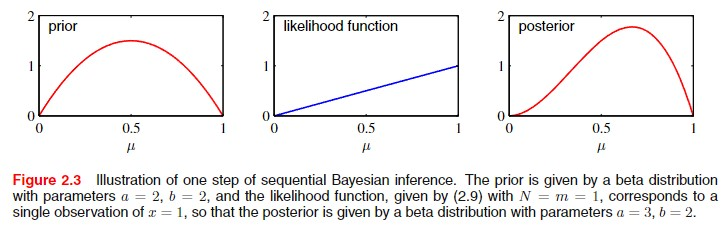
\includegraphics{bishop_23.jpg}
\end{figure}
\par
\textbf{Solução:}


%%%%%%%%%%%%%%%%%%%%%%%%%%%%%%%%%%%%%%%%%%%%%%%%%%%%%%%%%%%%%%%


\item \textbf{Verificação experimental do Teorema Central do Limite} \par
Considere a média de N variáveis aleatórias iid. Plote o histograma dessa média considerando que as N variáveis aleatórias têm a seguinte pdf:

1o caso: Uniforme(0,1) - uniforme no intervalo 0 a 1;

2o caso: Bernoulli - escolha o valor do parâmetro como quiser;

Note que, para N suficientemente grande, a distribuição da média converge para uma Gaussiana.

OBS: Usei média ao invés de soma para facilitar a geração do histograma (o eixo horizontal vai ficar fixo, facilitando a comparação para diferentes valores de N, igual na Figura 2.6 do livro).

\begin{figure}[H]
    \caption*{\textbf{Figura 2.6 do Bishop}}
       \centering
       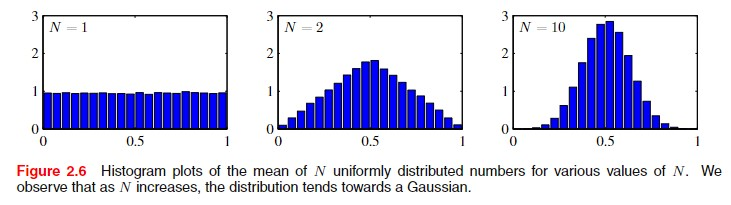
\includegraphics{bishop_26.jpg}
\end{figure}
\par
\textbf{Solução:}


%%%%%%%%%%%%%%%%%%%%%%%%%%%%%%%%%%%%%%%%%%%%%%%%%%%%%%%%%%%%%%%

\item \textbf{Verificação experimental da Law of Large Numbers - LLN} \par
Considere N variáveis aleatórias independentes geradas a partir de uma distribuição normal padrão (isto é, Gaussiana de média 0 e variância 1). Compute o estimador média amostral. Repita o experimento diversas vezes e plote o histograma desse estimador para um dado valor de N. Mostre que, conforme N aumenta, o histograma desse estimador fica cada vez mais estreito em torno do valor correto (i.e., variância vai diminuindo), que é zero.
\par
\textbf{Solução:}


%%%%%%%%%%%%%%%%%%%%%%%%%%%%%%%%%%%%%%%%%%%%%%%%%%%%%%%%%%%%%%%

\item \textbf{Estimação de pdf} \par
Tente replicar os resultados exibidos nas figuras 2.24 e 2.25 do livro. Para isso, gere uma amostra de N=50 dados cuja distribuição é dada pela curva em verde (corresponde a uma mistura de 2 gaussianas - veja equação 
$$p(x) = \sum_{k=1}^{K}\pi_k \mathcal{N} (x|\mu_k. \Sigma_k)$$ 
e escolha os parâmetros dessa distribuição da forma que quiser). Estime a pdf do modelo gerador dos dados utilizando 2 métodos: histograma e kernel Gaussiano. Para o parâmetro h, utilize os mesmos valores das figuras.
\begin{figure}[H]
    \caption*{\textbf{Figura 2.24 do Bishop}}
       \centering
       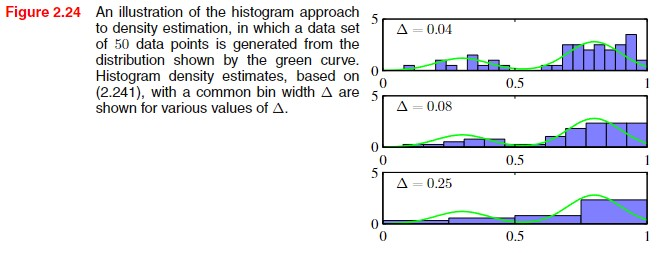
\includegraphics{bishop_224.jpg}
\end{figure}
\begin{figure}[H]
    \caption*{\textbf{Figura 2.25 do Bishop}}
       \centering
       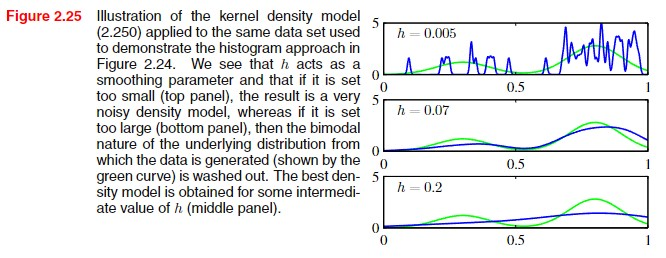
\includegraphics{bishop_225.jpg}
\end{figure}
\par
\textbf{Solução:}


%%%%%%%%%%%%%%%%%%%%%%%%%%%%%%%%%%%%%%%%%%%%%%%%%%%%%%%%%%%%%%%

\item \textbf{Classificador K-NN} \par
Considere 2 classes, C1 e C2, que correspondem aos seguintes modelos geradores: 

C1: pdf Gaussiana de média -1 e variância 1

C2: pdf Gaussiana de média 1 e variância 1

Gere 10 observações de cada uma dessas classes e assuma que você sabe exatamente a classe de cada um dos 20 pontos gerados (10 pontos para cada classe). Em seguida, gere mais 2 observações de cada classe e assuma que você NÃO sabe de qual classe esses novos dados pertencem. Utilize a técnica de K-NN, considerando diferentes valores de K, para classificar os 4 novos dados.

OBS: Plote os resultados utilizando cores e símbolos para facilitar a interpretação. Por exemplo: Para os 20 pontos conhecidos, represente-os usando `bolinhas' vermelhas para C1 e azuis para C2. Para os 4 pontos a serem classificados, mantenha o código de cores (para sabermos identificar qual era a classe correta) e use novos símbolos para identificar se a classificação foi correta (use um `quadrado') ou se a classificação foi errada (neste caso, use um `x').

Se for usar outros símbolos e cores, não tem problema. Só não esqueça de fazer uma
legenda ou caption que me permita compreender a figura.


\par
\textbf{Solução:}


%%%%%%%%%%%%%%%%%%%%%%%%%%%%%%%%%%%%%%%%%%%%%%%%%%%%%%%%%%%%%%%



\end{enumerate}
\appendix

\section*{Códigos}

\lstinputlisting[language=Python,caption=Exercício extra 1]{ex1.py}

\lstinputlisting[language=Python,caption=Exercício extra 2]{ex2.py}

\lstinputlisting[language=Python,caption=Exercício extra 3]{ex3.py}

\lstinputlisting[language=Python,caption=Exercício extra 4]{ex4.py}

\lstinputlisting[language=Python,caption=Exercício extra 5]{ex5.py}



\end{document}